\documentclass[a4paper, 12pt]{article}

% Extension des capacités
\usepackage{etex}

% Mise en page
% \usepackage[a4paper, left=1.5cm, right=1.5cm, top=2cm, bottom=2cm, heightrounded]{geometry}
\usepackage{polytechnique}

% Francisation du document
\usepackage[T1]{fontenc}
\usepackage[utf8]{inputenc}
\usepackage[frenchb]{babel}

\usepackage{float}
\usepackage{caption}

\usepackage{layout} % \layout au début de doc -> longueurs caractéristiques de la mise en page

\usepackage{lmodern}
\usepackage{eurosym}
\usepackage[french]{varioref}

\usepackage{amsmath, amsfonts, amssymb}
\usepackage{mathrsfs}

\usepackage{hyperref}
\usepackage{siunitx}
\sisetup{%
 unitsep = \cdot,%
 decimalsymbol = comma,%
 expproduct = \cdot,%
 seperr,%
 trapambigerr = false,%
 alsoload = hep%
}

\hypersetup{%
 pdftitle = {INF552 - Graphcut textures},%
 pdfsubject = {},%
 pdfkeywords = {},%
 pdfcreator = {pdfLaTeX},%
 pdfproducer = {pdfLaTeX},%
 bookmarksnumbered = true,%
 pdfstartview = FitH,%
 pdfpagelayout = OneColumn,%
 colorlinks = false,%
 pdfborder = {0 0 0}%
}

\usepackage{xcolor}
\usepackage[ensemblesGras]{mesfonctions}

\renewcommand{\thefootnote}{(\roman{footnote})}
\DeclareMathOperator{\sg}{sg}

\title{Graphcut Textures}
\subtitle{INF582}
\author{\textsc{Masset} Camille \\ \textsc{Shen} Yuesong \\ X2013}
\date{le \today}


\begin{document}
\renewcommand{\arraystretch}{1.5}
\newcommand{\grc}{\emph{graph cuts}}

\maketitle

\section{Rappel du sujet.}
L'article \emph{Graphcut Textures: Image and Video Synthesis Using Graph Cuts} présente une technique
pour synthétiser des textures à partir d'un petit échantillon, par exemple une étendue d'herbe ou une foule.

Une partie de l'échantillon est découpée selon un chemin optimal puis copiée sur l'image de sortie.
Cette méthode se base essentiellement sur une technique de \grc{}.


\section{Implémentation de GraphCut.}
L'image de sortie est associée à un graphe dans lequel chaque n\oe{}ud correspond à un pixel de l'image.
Les arêtes du graphes relient des n\oe{}uds correspondant à des pixels conjoints.

Pour les besoins de l'algorithme, on introduit une structure \verb|Cut| pour représenter un \emph{cut} précédent.
Cette structure comporte trois attributs:
\begin{itemize}
    \item \verb|double cost|: le coût du \emph{cut};
    \item \verb|Vec3b hiddenPix1|: le pixel qui a été masqué suite au \emph{cut};
    \item \verb|Vec3b hiddenPix2|: le pixel qui a été conservé visible suite au \emph{cut}.
\end{itemize}
On utilise alors deux tableaux de \verb|Cut|: un pour les coupes verticales et un pour les coupes horizontales.

Une fois la position du \emph{patch} d'entrée choisie (voir sectino suivante), on met à jour le graphe et on cherche le flot maximal.

Après avoir calculé le flot maximal, il faut déterminer les pixels à garder dans la zone de recouvrement entre le \emph{patch} et la sortie.
On met ensuite à jour les tableaux de \verb|Cut|s puis les pixels de la sortie.


\section{Positionnement des \emph{patches}.}
Avant d'appliquer la méthode de \grc{} à notre problème, il faut positionner un \emph{patch} de l'échantillon d'entrée.
Plusieurs méthodes sont présentées dans l'article et nous en avons implémentées deux:
une méthode complètement aléatoire et une méthode qui cherche à minimiser un coût sur toutes les positions possibles.

\subsection{Positionnement aléatoire.}
Cette méthode est la plus simple.
On choisit aléatoirement une translation de l'échantillon d'entrée sur la sortie et on applique la méthode de \grc{} qui sélectionne une partie de cette échantillon.
Cette méthode est plutôt rapide mais ne donne pas de très bons résultats si la texture est structurée (voir les exemples plus bas).

\subsection{Positionnement par minimisation globale du coût.}
On parcourt ici toutes les translations possibles de l'échantillon sur la sortie et on calcule le coût de cette translation.
Ensuite, on utilise ces coûts pour établir une distribution de probabilité sur les translations et on effectue un tirage pour déterminer la translation retenue.
Cette méthode est beaucoup plus coûteuse en temps que la précédente.

\subsection{Initialisation de la sortie.}
Pour simplifier l'implémentation, on ne part jamais d'une sortie vide: on y place naïvement l'échantillon d'entrée répété en quadrillage.
Afin de ne pas retenir les jonctions entre deux échantillons, on affecte un poids maximal, dans le graphe, entre deux pixels correspondant à des copies différentes de l'échantillon.
La zone de recouvrement entre un \emph{patch} et la sortie est donc toujours le \emph{patch} entier, donc une forme rectangulaire.


\section{Présentation des résultats.}
On a exécuté le programme sur différents types d'entrée.
On présente en figure~\vref{results} les résultats sur une image d'herbe (très aléatoire) et sur une image de fraises (plus structurée), avec le positionnement aléatoire.

Pour l'herbe, on a l'échantillon d'entrée, puis une vue des \emph{cuts} au cours de l'exécution de l'algorithme.
Enfin, on constate que le résultat final est plutôt bon, on ne distingue pas de coupures marquées dans l'image finale.

En revanche pour les fraises, le résultat final est moins bon: on voit des coupures au milieu des fruits.
Ceci est dû au fait que l'échantillon d'entrée possède une structure et que le positionnement aléatoire n'est pas adapté pour ce type d'entrée.
L'image du milieu montre l'initialisation de la sortie obtenue par juxtaposition de l'entrée.

\begin{figure}
    \begin{center}
        \null\hfill
        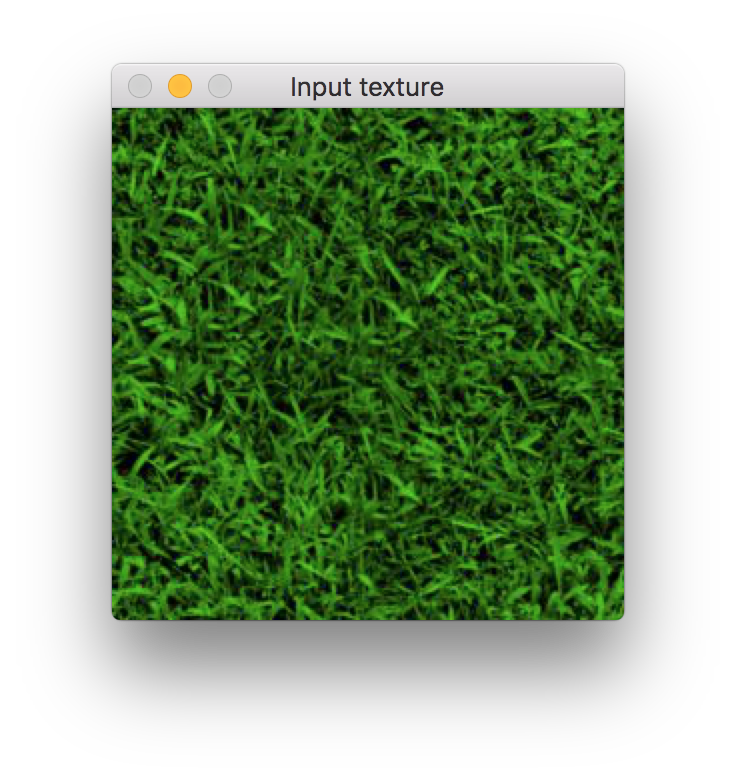
\includegraphics[width=0.3\textwidth]{images/grass_input}
        \hfill\hfill
        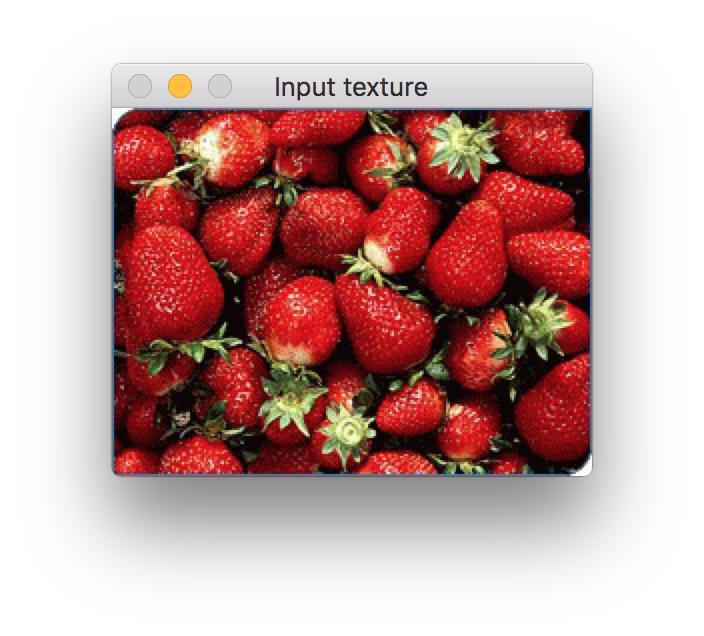
\includegraphics[width=0.3\textwidth]{images/strawberries_input}
        \hfill\null

        \null\hfill
        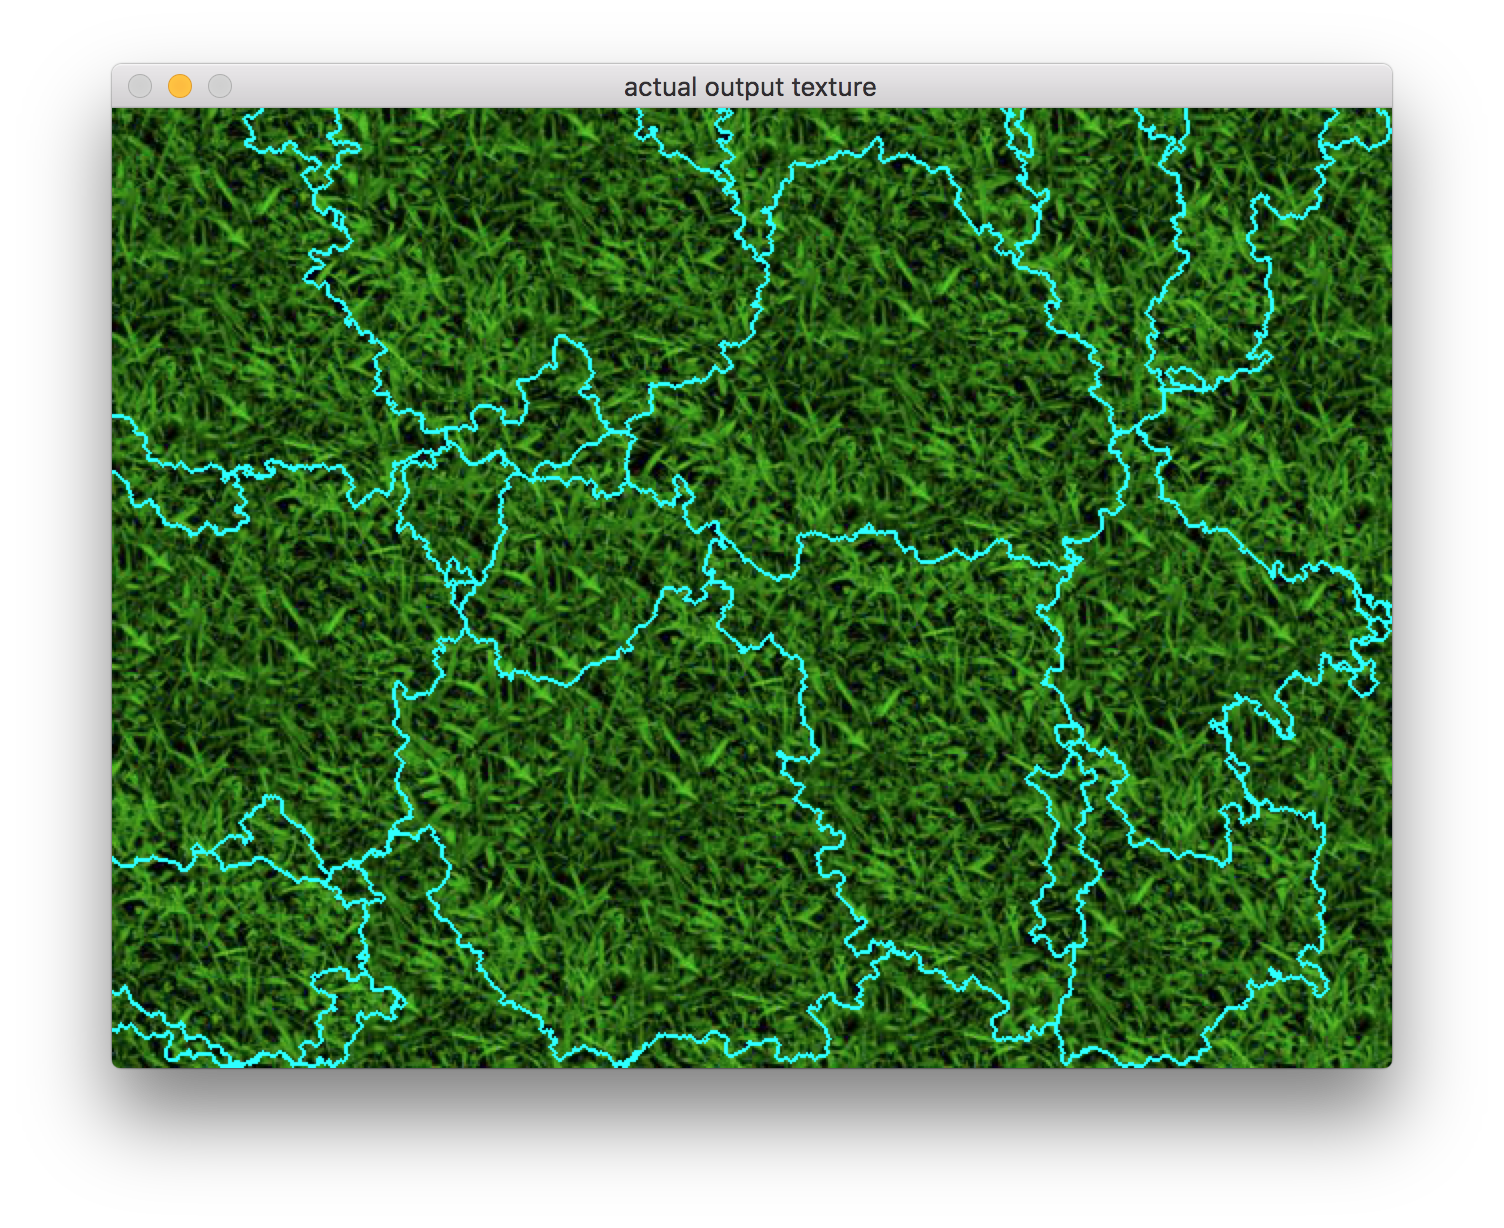
\includegraphics[width=0.45\textwidth]{images/grass_graphcuts}
        \hfill\hfill
        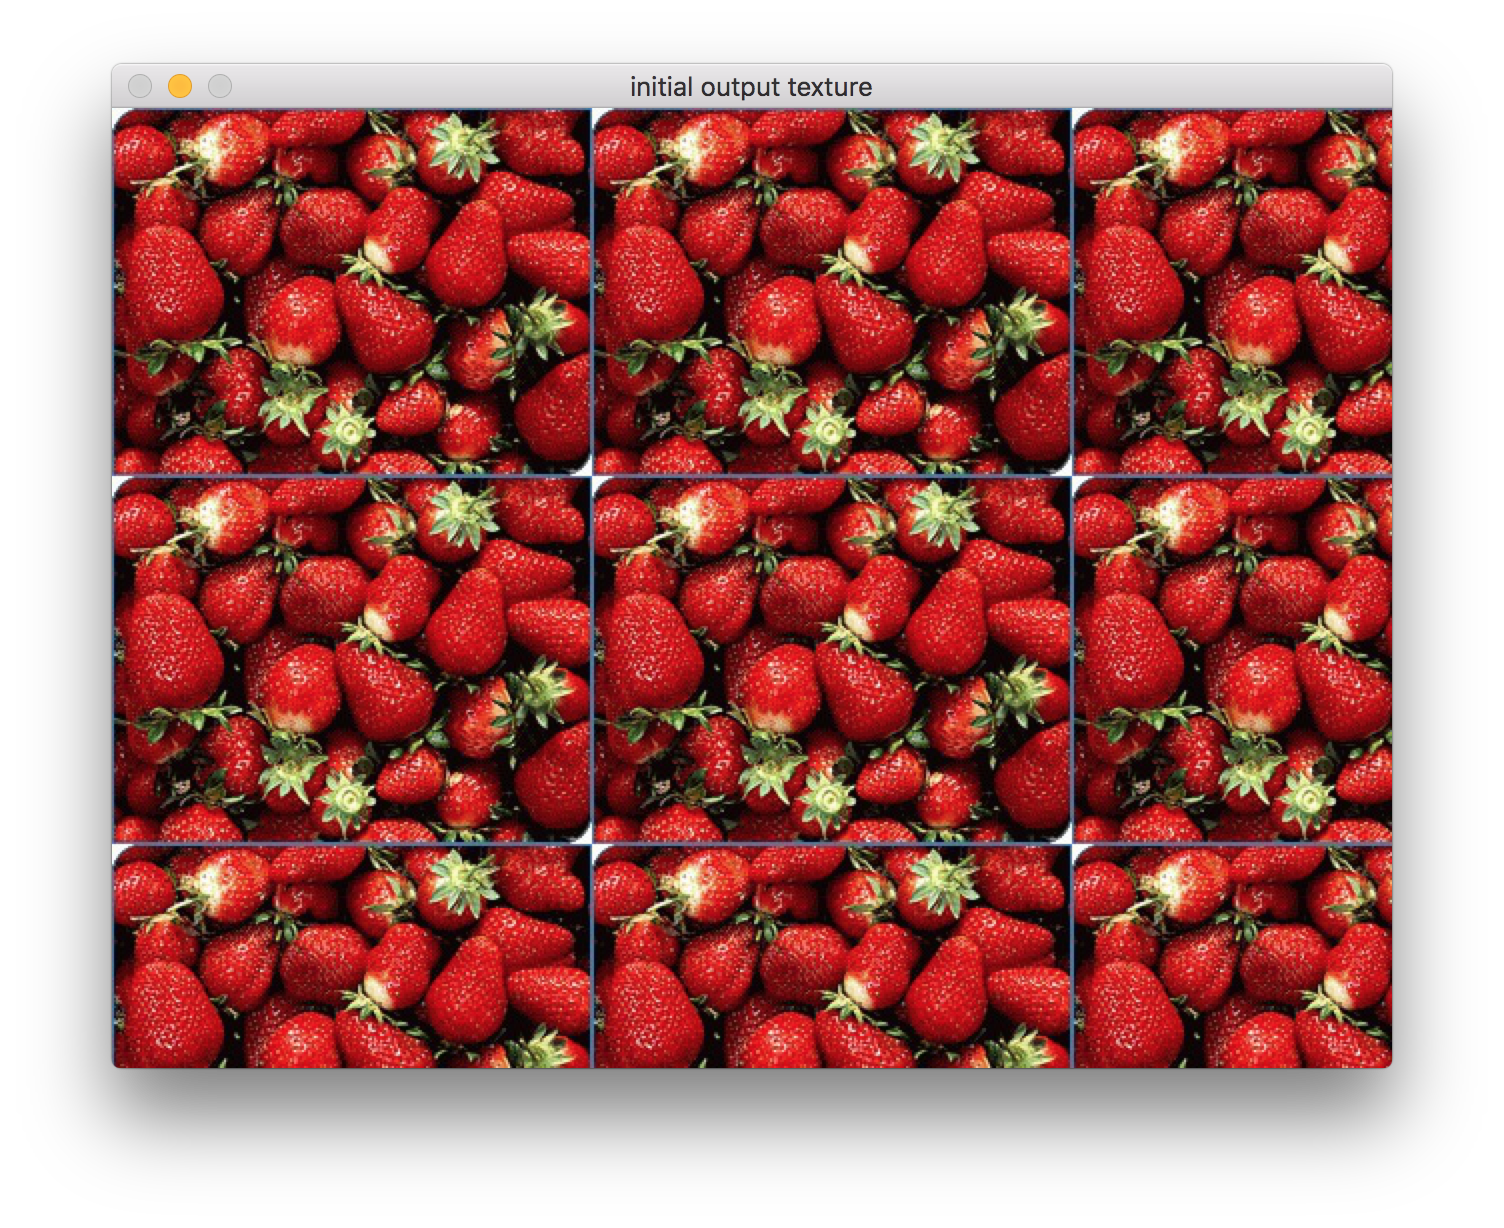
\includegraphics[width=0.45\textwidth]{images/strawberries_initial}
        \hfill\null

        \null\hfill
        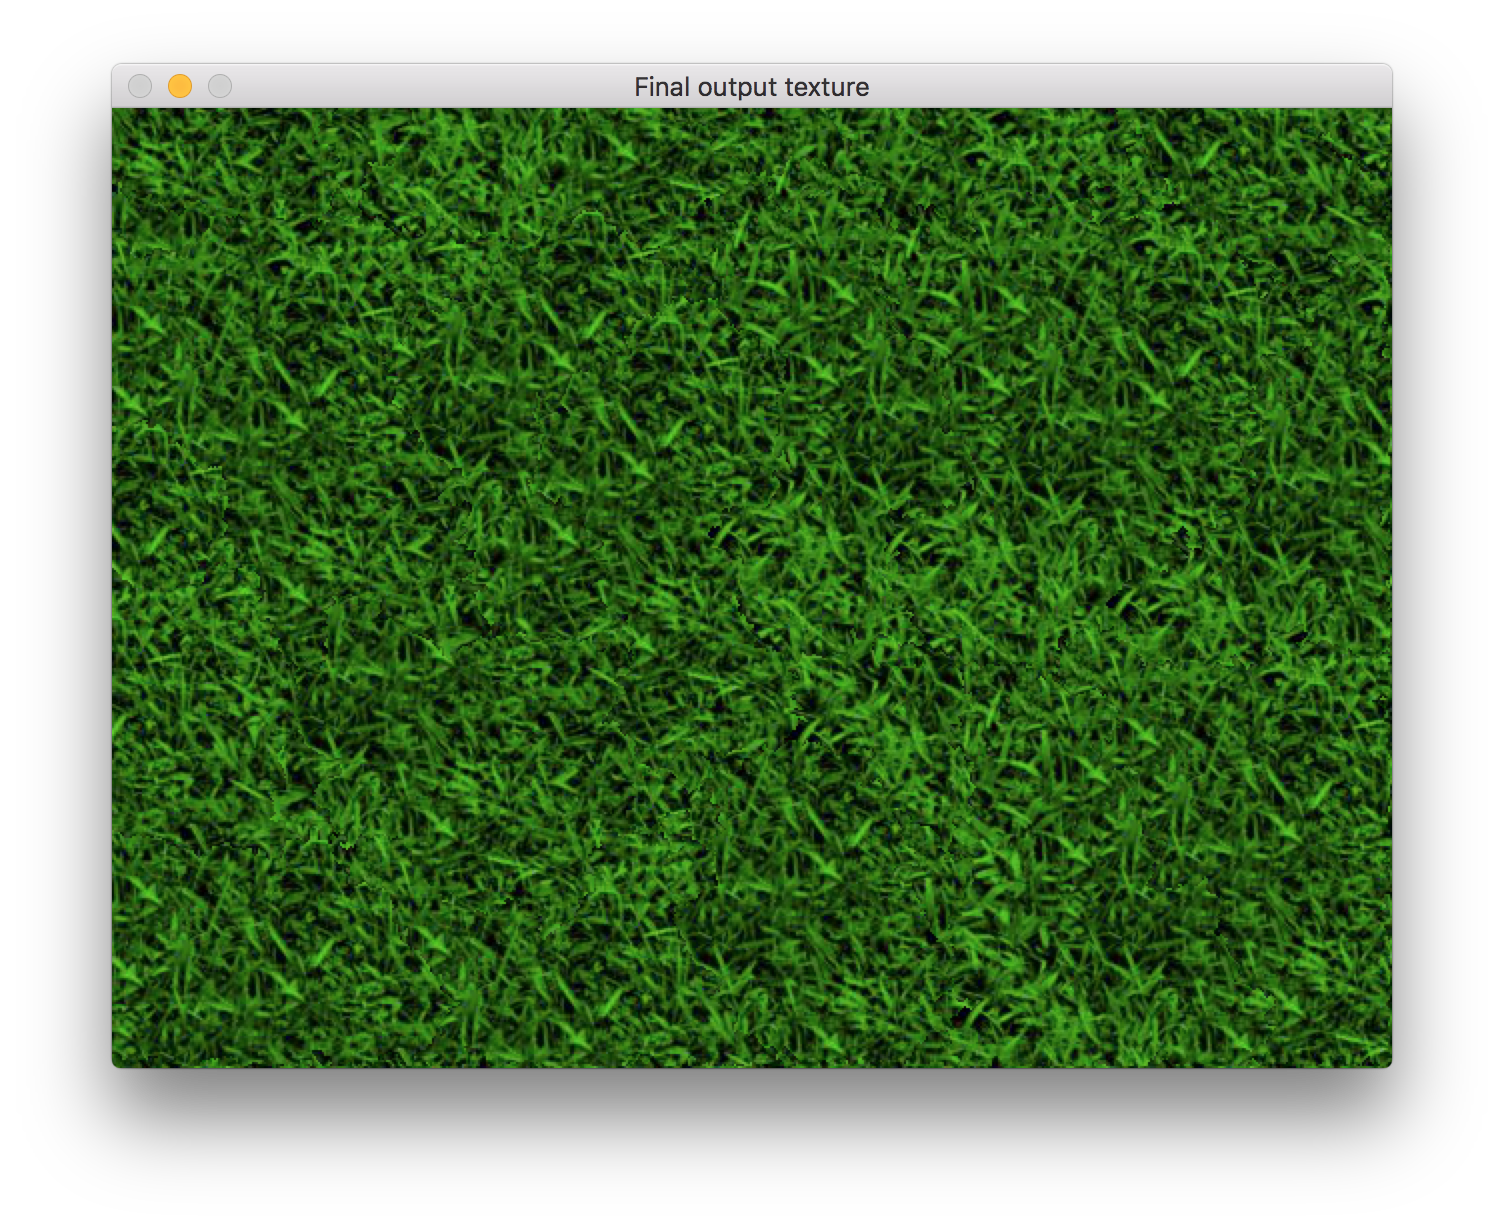
\includegraphics[width=0.45\textwidth]{images/grass_output}
        \hfill\hfill
        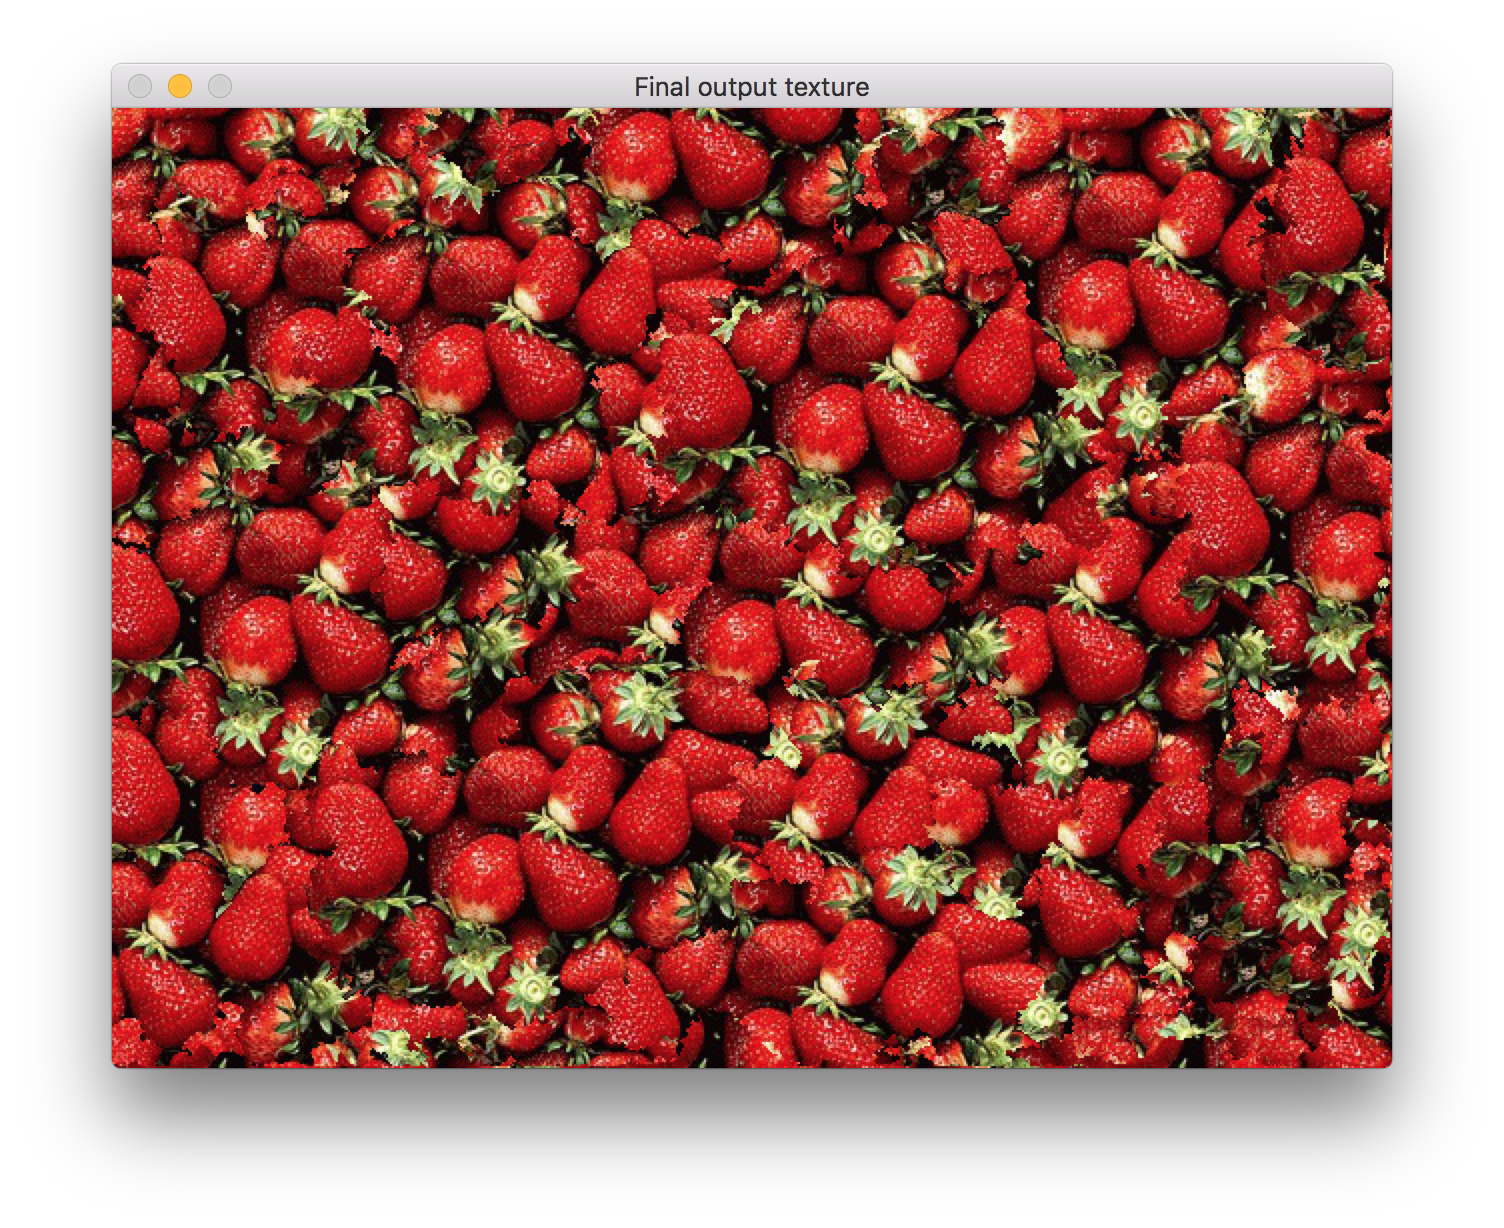
\includegraphics[width=0.45\textwidth]{images/strawberries_output}
        \hfill\null
    \end{center}
    \caption{Résultats obtenus avec l'herbe et les fraises.\label{results}}
\end{figure}

\end{document}
